\subsection{Relevanz von CB}
\label{sec:relevanz}
Benefits können in zweierlei Hinsicht gewinnbringend sein. Erstens sind sie ein gutes Mittel, um bestehende Mitarbeiter besser an das Unternehmen zu binden, indem sie deren Zufriedenheit und Loyalität erhöhen.\cite{werner2021strategic} Wenn Mitarbeiter das Gefühl haben, dass ihre Bedürfnisse und Wünsche durch verschiedene Leistungen erfüllt werden, sind sie eher bereit, länger im Unternehmen zu bleiben. Dies reduziert die Fluktuation und die damit verbundenen Kosten für Neueinstellungen und Einarbeitung. Zweitens sind Benefits ein wirksames Mittel, um einen größeren Kreis potenzieller neuer Mitarbeiter anzusprechen und das Unternehmen als attraktiven Arbeitgeber zu positionieren. Ein umfassendes Benefits-Programm kann das Interesse von Arbeitssuchenden wecken und dem Unternehmen helfen, sich von der Konkurrenz abzuheben, was die Rekrutierung von Talenten erleichtert.\cite{werner2021strategic} Darüber hinaus können Zusatzleistungen einen erheblichen Einfluss auf die Motivation und Produktivität der Mitarbeiter haben, indem sie ein Gefühl der Wertschätzung und Anerkennung vermitteln. Mitarbeiter, die sich durch Benefits unterstützt fühlen, sind oft motivierter und engagierter bei der Arbeit, was letztlich zu einer höheren Produktivität und besseren Geschäftsergebnissen führt.\cite{hong1995impact}.

\subsection{Benefits bei der Akquinet}
\label{sec:benefits}
Die Akquinet GmbH bietet ihren Mitarbeitern bereits eine Reihe von Benefits. Diese Benefits decken verschiedene Bereiche ab, die das Wohlbefinden und die Zufriedenheit der Mitarbeiter fördern sollen. Es sei darauf hingewiesen, dass die jeweiligen Vorteile von den jeweiligen Abteilungen, Standorten und Positionen abhängig sind.\cite{akquinetueberuns}\newline \newline
Zu den Benefits, welche den Mitarbeitern geboten werden, gehören unter anderem: \newline
\begin{itemize}
    \item \hyperref[sec:weiterbildung]{Weiterbildung}
    \item \hyperref[sec:mitarbeiterevents]{Mitarbeiter-Events}
    \item \hyperref[sec:felxarbeitszeiten]{Flexible Arbeitszeiten}
    \item \hyperref[sec:oepnvzuschuss]{ÖPNV Zuschuss}
    \item \hyperref[sec:betriebssport]{Betriebssport}
\end{itemize}
\cite{akquinetueberuns}

\subsubsection{Weiterbildung}\label{sec:weiterbildung}
In einer sich schnell wandelnden Welt ist es für Unternehmen von essenzieller Bedeutung, ihre Mitarbeitenden kontinuierlich weiterzubilden, um mit den neuesten Entwicklungen Schritt zu halten. Diesbezüglich genügt es nicht, allein theoretisches Wissen zu vermitteln.\cite{weiterbildungintro}\newline
Um die Effektivität der Weiterbildung zu optimieren, ist eine praktische Anwendung der erlernten Fähigkeiten unerlässlich. Dies gewährleistet, dass das Wissen nicht nur verstanden, sondern auch in der realen Arbeitswelt effektiv umgesetzt wird.\newline \newline
Des Weiteren ist ein effektiver Wissenstransfer zwischen den Mitarbeitenden von essenzieller Bedeutung. Der Austausch von Erfahrungen und Erkenntnissen innerhalb des Teams fördert die schnelle und umfassende Verbreitung neuer Kenntnisse. Dies führt nicht nur zu einer Steigerung der Qualität der Arbeitsergebnisse, sondern auch zu einer Stärkung der gesamten Organisation, da die Anpassungsfähigkeit und Innovationskraft erhöht werden.\cite{weiterbildungconc}\newline
Die erfolgreiche Integration dieser Aspekte resultiert in einer lernenden und anpassungsfähigen Organisation, die in der Lage ist, den Herausforderungen erfolgreich zu begegnen.\newline \newline
Die Akquinet GmbH hat mit dem Weiterbildungscampus (WEICA) innovative Weiterbildungsmöglichkeiten etabliert, die gezielt auf die Entwicklungsbedürfnisse ihrer Mitarbeitenden ausgerichtet sind. Das Schulungsangebot des WEICA ist umfassend und deckt sowohl technische als auch überfachliche Kompetenzen ab.\newline
Es basiert auf einer Kombination aus Präsenzseminaren und praxisorientierten Workshops, wodurch den unterschiedlichen Lernbedürfnissen der Teilnehmer entsprochen wird. Durch regelmäßige Aktualisierungen der Kursinhalte sowie kontinuierliche Evaluierungen gewährleistet WEICA, dass die Weiterbildungsmaßnahmen stets dem neuesten Stand entsprechen und die berufliche Entwicklung der Mitarbeitenden optimal unterstützt wird.\newline
Dies fördert nicht nur die individuelle Fachkompetenz und Karrierechancen der Mitarbeitenden, sondern stärkt auch die langfristige Innovationskraft und Wettbewerbsfähigkeit der Akquinet GmbH.

\subsubsection{Mitarbeiter-Events}\label{sec:mitarbeiterevents}
Mitarbeiter-Events stellen eine effektive Methode dar, um die Bindung der Mitarbeitenden an das Unternehmen zu vertiefen und deren positive Einstellung gegenüber der Firma zu fördern. Solche Veranstaltungen bieten nicht nur die Möglichkeit zur persönlichen Interaktion und zum Networking, sondern auch zur Stärkung des Gemeinschaftsgefühls und der Unternehmenskultur. Die informelle und entspannte Atmosphäre eines solchen Events ermöglicht den Mitarbeitenden, einander besser kennenzulernen und Beziehungen aufzubauen, was die Zusammenarbeit im Arbeitsalltag fördert.\cite{MAEvents}\newline \newline
Des Weiteren fördern Mitarbeiter-Events die Motivation und das Engagement der Mitarbeitenden. Die Wertschätzung der individuellen Beiträge sowie das Vorhandensein eines unterstützenden und wertschätzenden Umfelds wirken sich positiv auf die Leistung der Mitarbeitenden aus. Die gesteigerte Moral und das erhöhte Wohlbefinden der Mitarbeitenden haben häufig einen direkten Einfluss auf ihre Produktivität und Effizienz. In der Konsequenz lässt sich festhalten, dass gut organisierte Mitarbeiter-Events nicht nur die Mitarbeiterbindung stärken, sondern auch die Gesamtperformance und das Engagement der Belegschaft signifikant verbessern können.\cite{MAEvents}\newline \newline
Um detailliertere Erkenntnisse über die Mitarbeiter-Events der Akquinet GmbH zu gewinnen, wurden Gespräche mit drei Mitarbeitenden durchgeführt. Die Transkripte dieser Interviews sind in den Anhängen 1.0, 1.1 und 1.2 zu finden. \newline
Die Akquinet GmbH legt einen Fokus auf die Durchführung von Mitarbeiter-Events, mit dem Ziel, die Bindung der Mitarbeitenden an das Unternehmen zu intensivieren und eine positive Einstellung gegenüber der Firma zu fördern. In großen Unternehmen wie der Akquinet GmbH, in denen die Gefahr der Anonymität besteht, kommt derartigen Veranstaltungen eine besondere Bedeutung zu. (Siehe Anhang 1.0, Anhang 1.1, Anhang 1.2) Die jährlich stattfindende Weihnachtsfeier bietet den Mitarbeitenden eine wertvolle Gelegenheit, sich in einer entspannten Atmosphäre besser kennenzulernen und ihre Beziehungen untereinander zu vertiefen. (Siehe Anhang 1.1)\newline \newline
Des Weiteren werden regelmäßig teaminterne Events durchgeführt, die vom gemeinsamen Frühstücken bis zu Besuchen in Museen reichen. (Siehe Anhang 1.1) Diese regelmäßigen Veranstaltungen tragen nicht nur zur Stärkung des Gemeinschaftsgefühls und der Unternehmenskultur bei, sondern fördern auch die persönliche Interaktion und das Engagement der Mitarbeitenden. Durch diese Maßnahmen wird die Produktivität und Performance der Belegschaft nachhaltig unterstützt und gesteigert, und die Gefahr der Anonymität wird erfolgreich gemindert.

\subsubsection{Flexible Arbeitszeiten}\label{sec:felxarbeitszeiten}
Die Erfahrungen mit der globalen Pandemie des neuen Coronavirus haben gezeigt, dass flexible Arbeitszeiten und Arbeitsorte eine zentrale Rolle in der modernen Arbeitswelt spielen. Die Flexibilität bringt signifikante Vorteile mit sich, insbesondere für die physische Gesundheit der Mitarbeitenden.\cite{arbeitszeit}\newline
Einerseits wird der Stress reduziert, andererseits findet eine bessere Anpassung an individuelle Bedürfnisse statt. Dies resultiert in einer Reduktion der krankheitsbedingten Ausfälle und einer Steigerung der Arbeitsfähigkeit.\newline
Zudem begünstigt die Flexibilität eine ausgewogenere Work-Life-Balance, was zu einer höheren Zufriedenheit und Motivation der Mitarbeitenden beiträgt.\cite{arbeitszeit} Langfristig kann dies auch zu einer verbesserten Produktivität und einem positiveren Arbeitsumfeld führen. \newline \newline
Auch die Akquinet GmbH hat diese Erkenntnisse in ihre Unternehmenskultur integriert und bietet ihren Mitarbeitenden flexible Arbeitszeiten sowie die Möglichkeit, von verschiedenen Orten aus zu arbeiten. Dies erleichtert den Mitarbeitenden die Vereinbarkeit ihrer beruflichen und privaten Verpflichtungen und wirkt sich somit positiv auf ihre allgemeine Zufriedenheit aus.\newline
Allerdings birgt diese Flexibilität das Risiko, dass Mitarbeitende hauptsächlich außerhalb des Büros arbeiten und ihre Arbeitszeiten nicht mehr mit denen ihrer Kolleginnen und Kollegen übereinstimmen. Dies könnte zu einer Anonymisierung und einem Verlust an Teamzusammenhalt führen. Daher ist es von entscheidender Bedeutung, ein ausgewogenes Verhältnis zu finden, um die Vorteile der Flexibilität zu nutzen, ohne dabei die Teamdynamik zu beeinträchtigen.

\subsubsection{ÖPNV Zuschuss}\label{sec:oepnvzuschuss}
In Anbetracht der zunehmenden Umweltbelastungen und der steigenden CO2-Emissionen durch den Individualverkehr erlangt die Unterstützung alternativer, umweltfreundlicherer Transportmittel eine hohe Bedeutung.\cite{personalverkehr} \newline
Die Akquinet GmbH leistet hierzu einen Beitrag, indem sie die Nutzung öffentlicher Verkehrsmittel finanziell attraktiver gestaltet, was auf eine höheren Nutzung des ÖPNV schließen lässt. Diese Maßnahme fördert nicht nur die Mobilität der Belegschaft, sondern unterstützt auch das Ziel des Unternehmens, einen Beitrag zum Umweltschutz zu leisten. Eine Reduktion des motorisierten Individualverkehrs kann zu einer Verringerung der CO2-Emissionen und anderer schädlicher Abgase beitragen, welche maßgeblich zur Luftverschmutzung und zum Klimawandel beitragen.\newline
Die Bezuschussung von ÖPNV-Tickets durch Akquinet kann als Zeichen für das Engagement des Unternehmens im Bereich der nachhaltigen IT gewertet werden. Dies demonstriert, dass Nachhaltigkeit und ökologisches Bewusstsein sowohl in den offerierten IT-Lösungen als auch in den Geschäftsprozessen und der Mobilität der Mitarbeitenden integriert sind. Die Förderung umweltfreundlicher Mobilitätsalternativen reduziert die Umweltauswirkungen des Pendelns und trägt zur Förderung nachhaltiger Lebensweisen bei.

\subsubsection{Betriebssport}\label{sec:betriebssport}
In Berufen, die durch längere Sitzphasen gekennzeichnet sind, ist die Schaffung eines angemessenen physischen Ausgleichs von größter Bedeutung.\cite{langesitzen} Dies dient der Erhaltung der körperlichen Gesundheit der Mitarbeitenden und trägt zur Prävention von Haltungsschäden sowie muskulären Beschwerden bei.\cite{langesitzen} Die Förderung von Betriebssport kann zu einer Verbesserung der Gesundheit der Belegschaft und somit zu einer Reduktion von Krankheitsausfällen führen.\cite{betriebssportfördertgesundheit}\newline
Ein solcher Ansatz führt nicht nur zu einer Steigerung des Wohlbefindens der Mitarbeitenden, sondern kann auch die Produktivität und Effizienz innerhalb des Unternehmens erhöhen.\newline
Langfristig kann dies zudem die Attraktivität des Unternehmens als Arbeitgeber erhöhen und es wettbewerbsfähiger auf dem Arbeitsmarkt machen.\newline \newline
Die Akquinet GmbH offeriert ein umfassendes und vielseitiges Programm im Bereich Betriebssport, welches darauf abzielt, die körperliche Gesundheit der Mitarbeitenden zu fördern und präventiv gegen Haltungsschäden sowie muskuläre Beschwerden vorzugehen. Das Engagement für die Gesundheit und das Wohlbefinden der Mitarbeitenden stärkt deren Zufriedenheit und Produktivität und trägt zudem zur Attraktivität des Unternehmens als Arbeitgeber bei.\newline
Ein Betriebssportprogramm dieser Art stellt für potenzielle neue Mitarbeiter einen wesentlichen Attraktivitätsfaktor dar. Das Angebot unterscheidet sich positiv von dem anderer Arbeitgeber und kann somit effektiv zur Gewinnung neuer Talente genutzt werden. Indem das Unternehmen seine Investitionen in die Mitarbeitergesundheit betont, positioniert es sich als fortschrittlicher und fürsorglicher Arbeitgeber, der großen Wert auf das Wohl seiner Mitarbeiter legt und dadurch die Rekrutierung neuer Fachkräfte erleichtert.

\subsection{Metadaten der Umfrage}
Die empirische Erhebung erfolgte mittels des Umfrage-Tools Microsoft Forms. Die erstellten Abbildungen wurden mithilfe von PowerBI generiert. Der Fragebogen beinhaltete abschließende, offen gestellte Fragen sowie Fragen zum Net Promoter Score (NPS). Die Grundgesamtheit der Untersuchung umfasste 110 Personen.\newline 
Die befragten Personen wurden in fünf Altersgruppen aufgeteilt: Gruppe 1 umfasst die 15- bis 18-Jährigen, Gruppe 2 die 19- bis 24-Jährigen, Gruppe 3 die 25- bis 30-Jährigen, Gruppe 4 die 30- bis 40-Jährigen und Gruppe 5 Personen, die älter als 40 Jahre sind. Die zweite Gruppe umfasst etwa 70 \% der Befragten das ist in \hyperref[abb:alter]{Abbildung 1} dargestellt. Dies ist in erster Linie darauf zurückzuführen, dass die Umfrage überwiegend über den E-Mail-Verteiler der Universität verteilt wurde.\newline
Die Ergebnisse der empirischen Erhebung sind in Anhang 1.3 dokumentiert.

\begin{figure}[H]
    \centering
    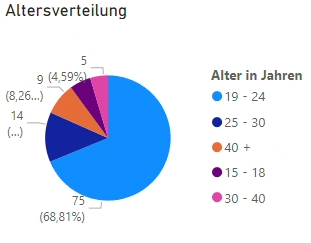
\includegraphics[scale = 0.7]{fig/Altersverteilung.png}
    \label{abb:alter}
    \caption{Altersverteilung}
\end{figure}

\subsection{Auswertung der Umfrage} \label{sec:auswertung}
Zu Beginn erfolgt eine Gegenüberstellung der neuen Ergebnisse mit den bereits bestehenden Benefits der Akquinet GmbH, die in \hyperref[sec:benefits]{Kapitel 2.2} ausführlich beschrieben wurden. Diese Gegenüberstellung dient der Identifikation von Übereinstimmungen sowie der Bewertung der zusätzlichen Mehrwerte der neuen Erkenntnisse. Die daraus gewonnenen Erkenntnisse werden genutzt, um gezielte Empfehlungen für die zukünftige Ausgestaltung der Benefits bei der Akquinet GmbH abzuleiten.

\subsubsection{Gegenüberstellung neuer Ergebnisse mit den bestehenden Benefits der Akquinet GmbH}
Wie in \hyperref[abb:weiterbildung]{Abbildung 2} ersichtlich, stellt die Relevanz von Weiterbildung in der befragten Gruppe einen zentralen Aspekt dar. Es lässt sich feststellen, dass für nahezu 84 \% der Befragten die persönliche Weiterentwicklung und Weiterbildung von höchster Bedeutung sind. Die hohe Priorität, die die Befragten der Weiterbildung beimessen, verdeutlicht die Relevanz kontinuierlicher Lern- und Entwicklungsprozesse in ihrem beruflichen und persönlichen Leben.\newline
In diesem Kontext nimmt die Akquinet GmbH eine bedeutsame Stellung ein, indem sie umfassende Weiterbildungsprogramme anbietet, welche bereits in \hyperref[sec:weiterbildung]{Kapitel 2.2.1} beschrieben wurden. Die genannten Programme fördern die Mitarbeiter durch gezielte Schulungen und Workshops kontinuierlich.\newline
Die Akquinet GmbH unterstützt damit nicht nur die individuelle Entwicklung, sondern stärkt auch das Unternehmen, indem sie das Wissen und die Qualifikationen der Belegschaft erhöht. Dies trägt zur Sicherstellung der Wettbewerbsfähigkeit in einem sich wandelnden Marktumfeld bei.
\begin{figure}[H]
    \centering
    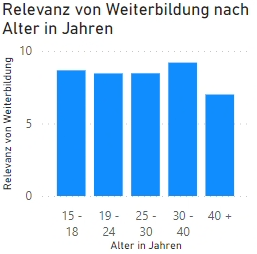
\includegraphics[scale = 0.7]{fig/Weiterbildung.png}
    \label{abb:weiterbildung}
    \caption{Relevanz von Weiterbildung}
\end{figure}

Die Relevanz von Hobbys für die Work-Life-Balance wird in \hyperref[abb:worklife]{Abbildung 3} ersichtlich. Die grafische Darstellung verdeutlicht, dass eine signifikante Mehrheit der Befragten Hobbys als essenziellen Faktor für ihr persönliches Wohlbefinden und ihre Zufriedenheit im Berufs- und Privatleben erachtet.\newline
Die Ausübung von Hobbys ermöglicht eine Reduktion von Stress und die Generierung von neuer Energie, was letztlich zu einer optimierten Balance zwischen Arbeit und Freizeit führt. Des Weiteren lässt sich anhand der Grafik ableiten, dass mit zunehmendem Alter eine Zunahme der Relevanz von Hobbys zu beobachten ist.\newline
Das Modell der flexiblen Arbeitszeiten und des variablen Arbeitsortes, welches von der Akquinet GmbH angeboten wird, in \hyperref[sec:felxarbeitszeiten]{Kapitel 2.2.3} beschrieben, stellt eine exzellente Ergänzung zu diesem Themenbereich dar. Die flexible Arbeitsgestaltung des Unternehmens zielt darauf ab, den Mitarbeitern die Anpassung ihrer Work-Life-Balance an die individuellen Bedürfnisse zu ermöglichen. Dies erlaubt den Beschäftigten, ihre beruflichen Verpflichtungen effizienter mit persönlichen und familiären Anforderungen zu vereinbaren, was zu einer gesteigerten Zufriedenheit und Produktivität führt.
\begin{figure}[H]
    \centering
    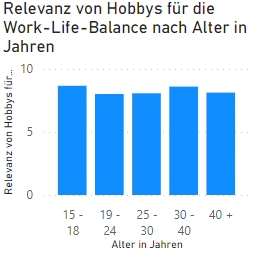
\includegraphics[scale = 0.7]{fig/work life.png}
    \label{abb:worklife}
    \caption{Relevanz von Hobbys für die Work-Life-Balance}
\end{figure}

Sozial- und Umweltthemen erfahren eine kontinuierliche Aufwertung, wie auch aus \hyperref[abb:umwelt]{Abbildung 4} ersichtlich wird. Über die Hälfte der Befragten gab an, ein Interesse an diesen Themen zu hegen. In diesem Kontext demonstriert die Akquinet GmbH ihr signifikantes Engagement für nachhaltige Mobilität durch die Einführung eines ÖPNV-Zuschusses, der bereits in \hyperref[sec:oepnvzuschuss]{Kapitel 2.2.4} detailliert erörtert wurde. Die Bezuschussung von ÖPNV-Tickets seitens der Akquinet GmbH verdeutlicht nicht nur das Interesse des Unternehmens an Umweltthemen, sondern stellt auch einen praktischen Beitrag zur Förderung nachhaltiger Mobilität dar. Dies manifestiert sich in der positiven Resonanz der Mitarbeitenden und führt zu einer Stärkung des Unternehmensimages in Bezug auf soziale Verantwortung.
\begin{figure}[H]
    \centering
    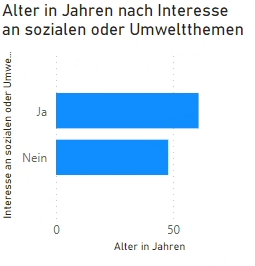
\includegraphics[scale = 0.7]{fig/umwelt.png}
    \label{abb:umwelt}
    \caption{Interesse an sozialen- oder Umweltthemen}
\end{figure}

Die Ergebnisse der Umfrage zur Relevanz von Sport im Privatleben lassen insgesamt eine eher neutrale Einschätzung erkennen. Dennoch lässt sich eine tendenzielle Zunahme der Bedeutung von Sport mit zunehmendem Alter feststellen, wie in \hyperref[abb:sport]{Abbildung 5} ersichtlich ist.\newline
Die Akquinet GmbH verfügt bereits über ein umfassendes Betriebssportangebot, dessen detaillierte Beschreibung in \hyperref[sec:betriebssport]{Kapitel 2.2.5} erfolgt. Das Angebot korrespondiert mit der zunehmenden Relevanz von Hobbys für die Work-Life-Balance. Die Beobachtung, dass Sport und Freizeitaktivitäten im Laufe des Lebens an Bedeutung gewinnen, lässt den Schluss zu, dass die Akquinet GmbH in vorteilhafter Weise aufgestellt ist, um den langfristigen Bedürfnissen und Interessen ihrer Mitarbeitenden gerecht zu werden. Dies führt zu einer Stärkung der Mitarbeiterbindung, da das Unternehmen nicht nur aktuelle, sondern auch zukünftige Interessen der Beschäftigten berücksichtigt.
\begin{figure}[H]
    \centering
    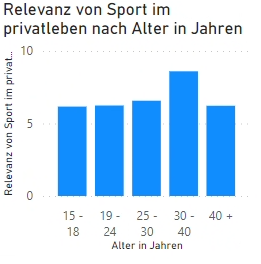
\includegraphics[scale = 0.7]{fig/sport.png}
    \label{abb:sport}
    \caption{Relevanz von Sport im Privatleben}
\end{figure}

\subsection{Handlungsempfehlung zu Corporate Benefits bei der Akquinet}
Es kann grundsätzlich festgestellt werden, dass die Akquinet GmbH bereits eine exzellente Ausgangslage aufweist, wie in \hyperref[sec:auswertung]{Kapitel 2.4} detailliert dargelegt wird. Das Unternehmen hat erkannt, dass die Förderung der Mitarbeiterzufriedenheit und -bindung durch CB von essenzieller Bedeutung ist, und hat ein umfassendes und gut durchdachtes Angebot entwickelt, das auf diese Bedürfnisse abgestimmt ist. Die gezielte Integration und kontinuierliche Verbesserung der CB-Programme demonstrieren, dass die Akquinet GmbH die Bedeutung dieser Maßnahmen verstanden hat und aktiv daran arbeitet, den Mitarbeitenden ein attraktives Arbeitsumfeld zu bieten.\newline \newline
Dennoch bestehen Möglichkeiten, das Angebot der Akquinet GmbH zu optimieren, insbesondere im Hinblick auf die Relevanz von Hobbys für die Work-Life-Balance. Obgleich das Unternehmen bereits über ein solides Benefits-Programm verfügt, könnte eine gezielte Mitarbeiterbefragung zusätzliche wertvolle Einblicke liefern. Eine derartige Umfrage würde es ermöglichen, die beliebtesten Freizeitaktivitäten und Interessen der Belegschaft mit hinreichender Präzision zu identifizieren. Dies eröffnet der Akquinet GmbH die Möglichkeit, spezifische Programme oder Anreize zu entwickeln, die auf die identifizierten Interessen zugeschnitten sind.\newline
Ein erweitertes Angebot, das den individuellen Vorlieben und Bedürfnissen der Mitarbeitenden Rechnung trägt, könnte nicht nur die Zufriedenheit und Motivation der Mitarbeitenden weiter steigern, sondern auch deren langfristige Bindung an das Unternehmen stärken. Durch die gezielte Ausrichtung des Angebots auf die gewünschten Freizeitaktivitäten kann die Work-Life-Balance der Mitarbeitenden weiter optimiert werden, wodurch das Unternehmen als attraktiver Arbeitgeber noch stärker positioniert wird.